\documentclass[12pt,a4paper]{report}
\usepackage[T2A]{fontenc}
\usepackage[utf8]{inputenc}
\usepackage[russian]{babel}
\usepackage[normalem]{ulem}
\usepackage{graphicx, setspace, amsmath, multirow}

\usepackage[
top = 1cm, 
bottom = 2.0cm,
left = 2cm,
right = 2cm
]{geometry}

\begin{document}
\scriptsize
\hspace{-1cm}
\begin{tabular}{p{11cm}}
    \vspace*{-1.3cm}
    \begin{center}
        \textbf{Санкт-Петербургский национальный исследовательский университет} \\ 
        \textbf{информационных технологий, механики и оптики} \\
        \hfill \\
        \textbf{УЧЕБНЫЙ ЦЕНТР ОБЩЕЙ ФИЗИКИ ФТФ}
    \end{center}
\end{tabular}
\hspace{0.5cm}
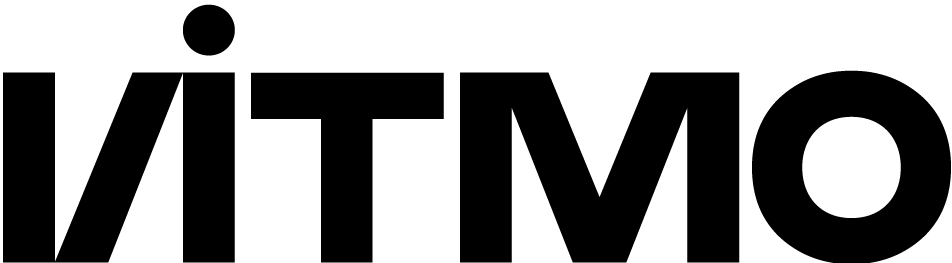
\includegraphics[width=5cm]{logo.png}
\normalsize
\begin{center}
    \line(1,0){500}
\end{center}
\begin{center}
    \begin{tabular}{ll}
        \textbf{Группа:} \uline{P3209 \hspace{5mm}\hfill} & \textbf{К работе допущен:} \uline{\hspace{4cm}} \\
        \textbf{Студент:} \uline{Степанов А.А. \hspace{5mm}\hfill} & \textbf{Работа выполнена:} \uline{\hfill} \\
        \textbf{Преподаватель:} \uline{Хвастунов Н.Н. \hspace{5mm}\hfill} & \textbf{Отчёт принят:} \uline{\hfill} \\
    \end{tabular}
\end{center}
\begin{center}
    \line(1,0){500}
\end{center}
\begin{center}
    \Huge
    Рабочий протокол и отчёт \\
    по лабораторной работе №3.10 \\
    \hfill\break
    \large
    \begin{tabular}{c}
        \textbf{ИЗУЧЕНИЕ СВОБОДНЫХ ЗАТУХАЮЩИХ} \\
        \textbf{ЭЛЕКТРОМАГНИТНЫХ КОЛЕБАНИЙ}
    \end{tabular}
\end{center}
\begin{center}
    \line(1,0){500}
\end{center}
\textbf{Цель работы:}
\begin{enumerate}
    \item Изучение основных характеристик свободных затухающих электромагнитных
    колебаний    
\end{enumerate}
\textbf{Задачи, решаемые при выполнении работы:}
\begin{enumerate}
    \item Вычисление значения логарифмического декремента $\lambda$
    \item Вычисление значения полного сопротивления $R$ и индуктивности $L$
    \item Вычисление добротности контура $Q$
    \item Построение графиков зависимостей
\end{enumerate}
\textbf{Объект исследования:}
\begin{enumerate}
    \item Свободные затухающие электромагнитные колебания
\end{enumerate}
\textbf{Метод экспериментального исследования:}
\begin{enumerate}
    \item Многократные измерения различных величин
\end{enumerate}
\textbf{Рабочие формулы и исходные данные:} \\
\hfill\break
\begin{tabular}{llll}
    $C_1=0.022uF$ & $C_2=0.033uF$ & $C_3=0.047uF$ & $C_4=0.47uF$ \\
    \hspace{4cm} & \hspace{4cm} & \hspace{4cm} & \hspace{4cm} \\
    $L=10mH$ & $\lambda=\dfrac{1}{n}\cdot\ln\ln\dfrac{U_i}{U_{i+1}}$ & $R=R_m+R_0$ & $Q=\dfrac{2\pi}{1-e^{-2\lambda}}$ \\
    \\
    $R_0=-R_m|_{\lambda=0}$ & $\lambda\approx\pi R\cdot\sqrt{\dfrac{C}{L}}$ & $Q=\dfrac{1}{R}\cdot\sqrt{\dfrac{L}{C}}$ & $R_{\text{crit}}=2\cdot\sqrt{\dfrac{L}{C}}$ \\
    \\
    $\delta T=\dfrac{T_\text{exp}-T_\text{th}}{T_\text{th}}$ & $T=\dfrac{2\pi}{\sqrt{\frac{1}{LC}-\frac{R^2}{4L^2}}}$ \\
\end{tabular}
\newpage\noindent
\textbf{Измерительные приборы:} \\
\hfill\break
\begin{tabular}{|c|c|c|c|c|}
    \hline
    & & & & \\
    № п/п & Наименование & Тип прибора & Используемый диапазон & Погрешность прибора \\
    & & & & \\
    \hline
    & & & & \\
    1. & Осциллограф & - & - & - \\
    & & & & \\
    \hline
\end{tabular} \\
\hfill\break
\hfill\break
\textbf{Схема установки:} \\
\begin{center}
    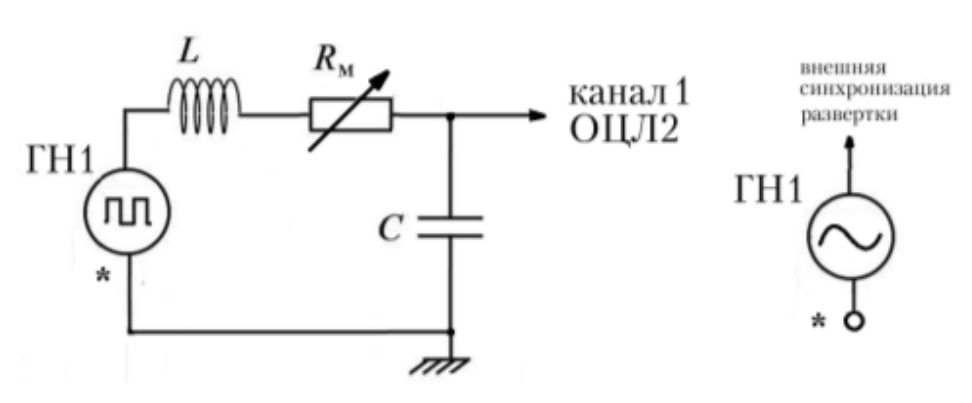
\includegraphics[width=10cm]{scheme.png}
\end{center}
\textbf{Результаты измерений и их обработки (таблицы, примеры расчетов):} \\
\hfill\break
\begin{tabular}{|c|c|c|c|c|c|c|c|c|c|c|c|}
    \hline
    $R_m$, Ohm & $T$, del & $T$, ms & $2U_i$, del & $2U_{i+n}$, del & $n$ & $\lambda$ & $Q$ & $R$, Ohm & $L$, mH \\
    \hline
    0 & 27.6 & 0.092 & 37 & 5 & 6 & 0.334 & 12.906 & 67 & 8.759 \\
    \hline
    10 & 27.6 & 0.092 & 37 & 4 & 6 & 0.371 & 11.999 & 77 & 9.365 \\
    \hline
    20 & 27.6 & 0.092 & 36.3 & 3 & 6 & 0.416 & 11.132 & 87 & 9.518 \\
    \hline
    30 & 23 & 0.092 & 35.9 & 3.5 & 5 & 0.466 & 10.370 & 97 & 9.424 \\
    \hline
    40 & 23 & 0.092 & 35.8 & 2.8 & 5 & 0.510 & 9.830 & 107 & 9.570 \\
    \hline
    50 & 18.4 & 0.092 & 35.3 & 4 & 4 & 0.544 & 9.472 & 117 & 10.029 \\
    \hline
    60 & 18.4 & 0.092 & 35 & 3 & 4 & 0.614 & 8.884 & 127 & 9.284 \\
    \hline
    70 & 13.8 & 0.092 & 34.8 & 4.7 & 3 & 0.667 & 8.528 & 137 & 9.151 \\
    \hline
    80 & 13.8 & 0.092 & 34.2 & 4 & 3 & 0.715 & 8.258 & 147 & 9.170 \\
    \hline
    90 & 9.2 & 0.092 & 33.9 & 7.4 & 2 & 0.761 & 8.038 & 157 & 9.243 \\
    \hline
    100 & 9.2 & 0.092 & 33.5 & 6.7 & 2 & 0.805 & 7.854 & 167 & 9.351 \\
    \hline
    200 & 4.6 & 0.092 & 30.8 & 8.6 & 1 & 1.276 & 6.814 & 267 & 9.511 \\
    \hline
    300 & 4.6 & 0.092 & 28.4 & 4.8 & 1 & 1.778 & 6.468 & 367 & 9.253 \\
    \hline
    400 & 4.6 & 0.092 & 26.2 & 2.4 & 1 & 2.390 & 6.336 & 467 & 8.288 \\
    \hline
\end{tabular}\\
\hfill\break
Конвертация $T$, del в $T$, ms: \\
$s_1$ - число маленьких делений в одном большом, $s_1=5$ \\
$n$ - количество делений \\
$s_2$ - количество секунд в большом делении, $s_2=100\cdot10^{-6}s$ \\
$10^3$ - количество миллисекунд в секунде \\
\hfill\break
$T_{ms}=\dfrac{T_\text{del}}{s_1\cdot n}\cdot s_2\cdot10^3$ \\
\hfill\break
\hfill\break
\begin{tabular}{|c|c|c|c|c|c|c|c|}
    \hline
    C & $T_\text{exp}$, del & $T_\text{exp}$, ms & $T_\text{th}$, ms & $\delta T$, \% & $\text{Thompson}$, ms & $\Omega_0$, hz & $\beta$ \\
    \hline
    C1 & 4.8 & 0.096 & 0.090 & 6.523 & 0.0901 & 67419.986 & \multirow{4}{*}{3350} \\
    \cline{1-7}
    C2 & 5.8 & 0.116 & 0.110 & 5.096 & 0.1104 & 55048.188 & \\
    \cline{1-7}
    C3 & 6.8 & 0.136 & 0.132 & 3.246 & 0.1317 & 46126.560 & \\
    \cline{1-7}
    C4 & 22 & 0.44 & 0.417 & 5.630 & 0.4165 & 14586.499 & \\
    \hline
\end{tabular}\\
\hfill\break
\textbf{Результаты различных величин, полученных в результате обработки данных:} \\
\hfill\break
\begin{tabular}{lll}
    $L_\text{avg}=9.351$ mH & $R_\text{cr}=1348.4$ Ohm & $R_0=67$ Ohm \\
    \hspace{5cm} & \hspace{5cm} & \hspace{5cm} \\
    $T=0.093$ ms, $R=R_0+R_m(0)$ \\
    \hspace{5cm} & \hspace{5cm} & \hspace{5cm} \\
    $T=0.093$ ms, $R=R_0+R_m(200)$ \\
    \hspace{5cm} & \hspace{5cm} & \hspace{5cm} \\
    $T=0.093$ ms, $R=R_0+R_m(400)$ \\
    \hspace{5cm} & \hspace{5cm} & \hspace{5cm} \\
    $Q=9.418$, $R = R_0+R_m(0)$ \\
    \hspace{5cm} & \hspace{5cm} & \hspace{5cm} \\
    $Q=8.473$, $R = R_0+R_m(10)$ \\
\end{tabular} \\
\hfill\break
\hfill\break
\textbf{Расчет погрешностей:} \\
\hfill\break
Среднее квадратичное отклонение: $\sigma=0.391$ \\
Коэффициент Стьюдента: $t_\alpha=\dfrac{\Delta L\cdot\sqrt{N}}{\sigma}=2.47\Rightarrow \alpha=0.99$
\begin{enumerate}
    \item $T_\text{exp}=0.096$, $T_\text{th}=0.090$, $\delta T=6.53\%$
    \item $T_\text{exp}=0.116$, $T_\text{th}=0.11$, $\delta T=5.096\%$
    \item $T_\text{exp}=0.136$, $T_\text{th}=0.132$, $\delta T=3.246\%$
    \item $T_\text{exp}=0.44$, $T_\text{th}=0.417$, $\delta T=5.63\%$
\end{enumerate}
\hfill\break
\textbf{Полученные графики:} \\
\hfill\break
Зависимость логарифмического декремента от сопротивления: \\
\begin{center}
    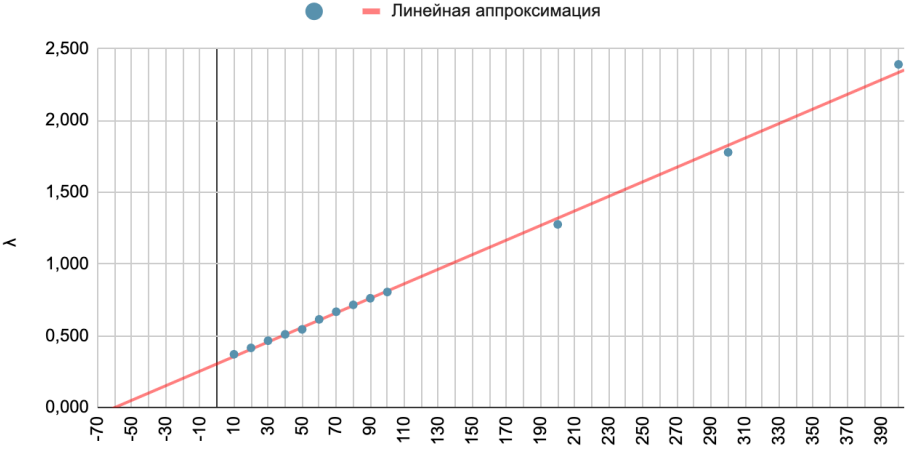
\includegraphics[width=\textwidth]{graph1.png}
\end{center}
\newpage\noindent
Зависимость добротности от сопротивления: \\
\begin{center}
    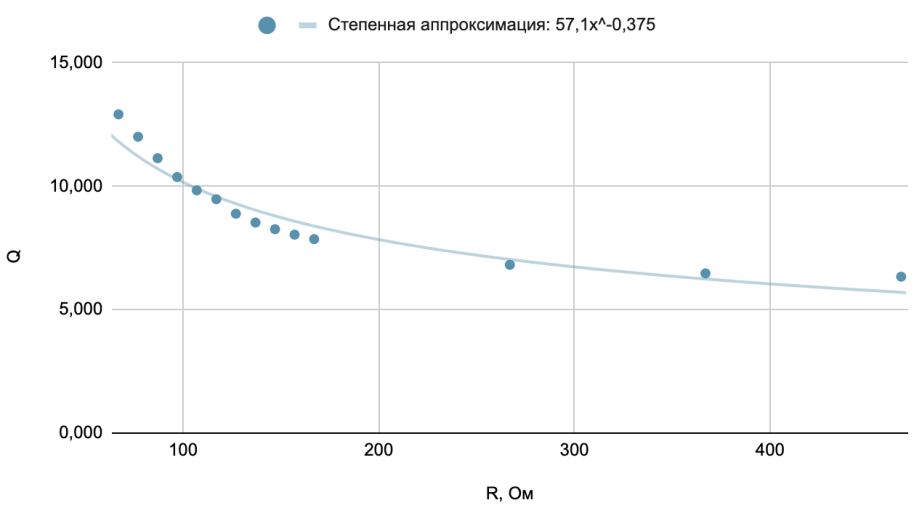
\includegraphics[width=\textwidth]{graph2.png}
\end{center}
Зависимость теоретического и экспериментального периодов от ёмкости конденсатора: \\
\begin{center}
    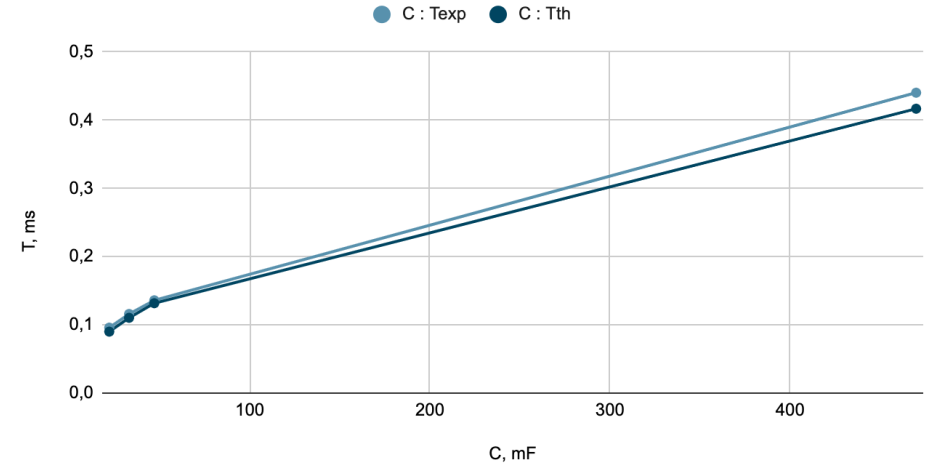
\includegraphics[width=\textwidth]{graph3.png}
\end{center}
\hfill\break
\textbf{Выводы и анализ результатов работы:} \\
\hfill\break
Были изучены основные характеристики свободных затухающих электромагнитных
колебаний, а также характер протекания колебаний в
контуре. Построены графики взаимных зависимостей. Была доказана
достоверность формулы Томпсона.
\end{document}